\documentclass[11pt,a4paper]{article}

\usepackage[utf8]{inputenc}
\usepackage[T1]{fontenc}
\usepackage{amsmath,amssymb,amsfonts}
\usepackage{physics}
\usepackage{hyperref}
\usepackage{booktabs}
\usepackage{geometry}
\usepackage{enumitem}
\usepackage{listings}
\usepackage{xcolor}
\usepackage{graphicx}
\usepackage{subcaption}

\geometry{margin=1in}
\hypersetup{colorlinks=true, linkcolor=blue, urlcolor=blue, citecolor=blue}

\lstset{
  language=Python,
  basicstyle=\ttfamily\small,
  keywordstyle=\color{blue},
  commentstyle=\color{gray},
  stringstyle=\color{red!70!black},
  showstringspaces=false,
  frame=single,
  breaklines=true,
}

\title{Derivation and Implementation Notes\\
\large Yi, Huo, Liu, Fan, Zhang \& Cao --- TTITE Algorithm\\
\normalsize EPJ Quantum Technology 12:43 (2025)}

\author{Companion document for the \texttt{quarksim} codebase}
\date{}

\begin{document}
\maketitle

\tableofcontents
\newpage

%=============================================================================
\section{The Core Idea: Imaginary-Time Evolution}
%=============================================================================

\subsection{Why Imaginary Time?}

Given a Hamiltonian $H$ with ground state $\ket{E_0}$ and eigenvalue $E_0$, the imaginary-time evolution operator $e^{-H\tau}$ preferentially amplifies the lowest-energy component of any initial state:
\begin{equation}
  \ket{\psi(\tau)} = A(\tau)\, e^{-H\tau}\ket{\psi(0)}
  \label{eq:ite}
\end{equation}
where $A(\tau)$ is a normalization constant. Since each eigenstate $\ket{E_k}$ is damped by $e^{-E_k \tau}$, the ground state (smallest $E_k$) dominates as $\tau \to \infty$.

The imaginary-time Schr\"odinger equation is (Eq.~1 of the paper):
\begin{equation}
  -\frac{d\ket{\psi}}{d\tau} = H\ket{\psi}
  \label{eq:ite_schrodinger}
\end{equation}

\textbf{The challenge:} $e^{-H\tau}$ is \textbf{non-unitary}---it cannot be directly implemented as a quantum gate. The TTITE algorithm overcomes this using Trotter decomposition, Taylor expansion, and ancilla-qubit postselection.


%=============================================================================
\section{Test Systems}
%=============================================================================

\subsection{Hydrogen Molecule (Eq.~12)}

The H$_2$ molecular Hamiltonian in the STO-3G basis, after Jordan-Wigner transformation and qubit reduction to 2 qubits:
\begin{equation}
  H_{\mathrm{H}_2} = c_0(D)\, I \otimes I
    + c_1(D)\, Z \otimes I
    + c_2(D)\, I \otimes Z
    + c_3(D)\, Z \otimes Z
    + c_4(D)\, X \otimes X
  \label{eq:h2}
\end{equation}
where the coefficients $c_i(D)$ depend on the interatomic distance $D$.

\textbf{Parameters (Table~\ref{tab:h2}):} The coefficients are computed from PySCF (RHF + molecular orbital integrals), mapped to a 2-qubit Hamiltonian via the FCI singlet/triplet block structure.

\begin{table}[h]
\centering
\begin{tabular}{llll}
\toprule
$D$ (\AA) & $c_0$ & $c_1 = c_2$ & $c_4$ \\
\midrule
0.35 & 0.701 & $-0.747$ & 0.163 \\
0.735 & $-0.332$ & $-0.398$ & 0.181 \\
\bottomrule
\end{tabular}
\caption{Selected H$_2$ Hamiltonian coefficients ($c_3$ is small, $\sim 0.01$).}
\label{tab:h2}
\end{table}

\noindent\textbf{Code:} \texttt{hamiltonian.h2\_coefficients(D)} interpolates from a 47-entry table computed via PySCF.

\subsection{Heisenberg Spin-1/2 Chain (Eq.~13)}

\begin{equation}
  H_{\mathrm{Heisenberg}} = -J\sum_{j=1}^{n-1}
    \left(\sigma_x^j\sigma_x^{j+1} + \sigma_y^j\sigma_y^{j+1} + \sigma_z^j\sigma_z^{j+1}\right)
    - h\sum_{j=1}^{n}\sigma_z^j
  \label{eq:heisenberg}
\end{equation}
where $J$ is the coupling strength, $h$ is the static magnetic field, and open boundary conditions are used.

\noindent\textbf{Code:} \texttt{hamiltonian.build\_heisenberg\_hamiltonian(n, J, h)}.

\subsection{Initial States}

Both systems use $\ket{+}^{\otimes n}$ as the initial state, which has a finite overlap with the ground state. For Figure~3, a biased initial state $(4\ket{00} + \ket{01} + \ket{10} + \ket{11})/\sqrt{19}$ is used.


%=============================================================================
\section{Trotter Decomposition (Eq.~2)}
%=============================================================================

For $H = \sum_{i=1}^{m} c_i h_i$ (sum of Pauli product terms), the Trotter approximation decomposes:
\begin{equation}
  e^{-H\tau} = \left(e^{-c_1 h_1 \Delta\tau} \cdots e^{-c_m h_m \Delta\tau}\right)^{L} + O(\Delta\tau)
  \label{eq:trotter}
\end{equation}
where $\Delta\tau$ is the Trotter step duration and $L = \tau/\Delta\tau$ is the number of segments.

Each factor $S(\Delta\tau) = \prod_i e^{-c_i h_i \Delta\tau}$ is called a \textbf{Trotter segment}, and each $T_i(\Delta\tau) = e^{-c_i h_i \Delta\tau}$ is a \textbf{Trotter step}.

The Trotter error is $O(\Delta\tau)$ per segment. As shown in the paper's Figure~6, this is the dominant source of error---the Taylor expansion error is negligible in comparison.

\noindent\textbf{Code:} \texttt{evolution.apply\_trotter\_segment\_matrix()} iterates over all Hamiltonian terms.


%=============================================================================
\section{Taylor Expansion and LCU (Eqs.~4--5)}
%=============================================================================

\subsection{The Key Simplification: $h_i^2 = I$}

Since each $h_i$ is a Pauli product (tensor product of $\{I, X, Y, Z\}$), we have $h_i^2 = I$. This means the Taylor series of $e^{-c_i h_i \Delta\tau}$ collapses:
\begin{equation}
  T_i^R(\Delta\tau) = \sum_{j=0}^{R} \frac{(-c_i \Delta\tau)^j}{j!}\, h_i^j
  = \underbrace{\sum_{\substack{j=0\\j\text{ even}}}^{R} \frac{(-c_i \Delta\tau)^j}{j!}}_{\alpha}\; I
  + \underbrace{\sum_{\substack{k=0\\k\text{ odd}}}^{R} \frac{(-c_i \Delta\tau)^k}{k!}}_{\beta}\; h_i
  \label{eq:taylor}
\end{equation}

So $T_i(\Delta\tau) \approx \alpha I + \beta h_i$ --- a linear combination of just \textbf{two} unitaries ($I$ and $h_i$).

When $R \to \infty$: $\alpha \to \cosh(c_i\Delta\tau)$ and $\beta \to -\sinh(c_i\Delta\tau)$.

\vspace{0.3em}
\noindent\textbf{Code:} \texttt{circuit.taylor\_coefficients(c\_i, dt, order)} computes $(\alpha, \beta)$.

\subsection{Matrix-Based Application}

In our statevector simulation, each Trotter step simply applies:
\begin{equation}
  \ket{\psi'} = (\alpha I + \beta h_i)\ket{\psi}, \qquad
  \ket{\psi_{\text{norm}}} = \frac{\ket{\psi'}}{\|\ket{\psi'}\|}
\end{equation}

Since $\alpha I + \beta h_i$ preferentially dampens high-energy eigenstates of $h_i$ (relative to the sign of $c_i$), the product of all Trotter steps across all terms drives the state toward the ground state of $H$.

\vspace{0.3em}
\noindent\textbf{Code:} \texttt{evolution.apply\_trotter\_step\_matrix()}.


%=============================================================================
\section{Quantum Circuit Implementation (Algorithm~1)}
%=============================================================================

On a quantum computer, the non-unitary operator $\alpha I + \beta h_i$ is implemented using one \textbf{ancilla qubit} and the Linear Combination of Unitaries (LCU) technique.

\subsection{The 4-Step Circuit}

\begin{enumerate}[nosep]
  \item \textbf{Encoding:} Apply $R_y(\theta)$ on the ancilla, where $\theta = 2\arccos\!\left(\frac{\alpha}{\sqrt{\alpha^2+\beta^2}}\right)$:
  \begin{equation}
    \ket{\phi_1} = \left(\frac{\alpha}{\sqrt{\alpha^2+\beta^2}}\ket{0} + \frac{\beta}{\sqrt{\alpha^2+\beta^2}}\ket{1}\right)\ket{\psi}
  \end{equation}

  \item \textbf{Controlled-$h_i$:} Apply $CU = \ket{0}\!\bra{0}\otimes I + \ket{1}\!\bra{1}\otimes h_i$:
  \begin{equation}
    \ket{\phi_2} = \frac{1}{\sqrt{\alpha^2+\beta^2}}\left(\alpha\ket{0}\ket{\psi} + \beta\ket{1}h_i\ket{\psi}\right)
  \end{equation}
  Since $h_i$ is a Pauli product, $CU$ decomposes into controlled-$X$, controlled-$Y$, controlled-$Z$ gates.

  \item \textbf{Hadamard:} Apply $H$ on the ancilla:
  \begin{equation}
    \ket{\phi_3} = \frac{1}{\sqrt{2(\alpha^2+\beta^2)}}\left[\ket{0}(\alpha I + \beta h_i)\ket{\psi} + \ket{1}(\alpha I - \beta h_i)\ket{\psi}\right]
  \end{equation}

  \item \textbf{Measure:} If ancilla = $\ket{0}$, the work system collapses to $(\alpha I + \beta h_i)\ket{\psi}$ (normalized).
\end{enumerate}

\subsection{Success Probability (Eq.~11)}

The probability of obtaining $\ket{0}$ on the ancilla is:
\begin{equation}
  P_s = \frac{1}{2(\alpha^2+\beta^2)}\|(\alpha I + \beta h_i)\ket{\psi}\|^2
  \label{eq:success_prob}
\end{equation}

\textbf{Lemma~1:} The success probability is monotonically increasing---$P(\Delta\tau) \leq P(2\Delta\tau) \leq \cdots \leq P(L\Delta\tau)$.

\vspace{0.3em}
\noindent\textbf{Code:} \texttt{circuit.build\_trotter\_step\_circuit()} builds the full LCU circuit for one step.


%=============================================================================
\section{Improved Circuit (Section~5, Fig.~7)}
%=============================================================================

The standard circuit's success probability can be improved by replacing the Hadamard in Step~3 with $R_y(\theta')^\dagger$, where:
\begin{equation}
  \theta' = 2\arccos\!\left(\sqrt{\frac{\alpha}{\alpha+\beta}}\right)
  \label{eq:improved_theta}
\end{equation}

The improved success probability is:
\begin{equation}
  P'_s = \frac{1}{(\alpha+\beta)^2}\|T_i(\Delta\tau)\ket{\psi}\|^2 \geq P_s
  \label{eq:improved_prob}
\end{equation}
since $(\alpha+\beta)^2 \leq 2(\alpha^2+\beta^2)$.

\vspace{0.3em}
\noindent\textbf{Code:} \texttt{circuit.build\_improved\_trotter\_step\_circuit()}.


%=============================================================================
\section{Results}
%=============================================================================

\subsection{H$_2$ Molecule: Convergence (Figure~2)}

\begin{figure}[h]
\centering
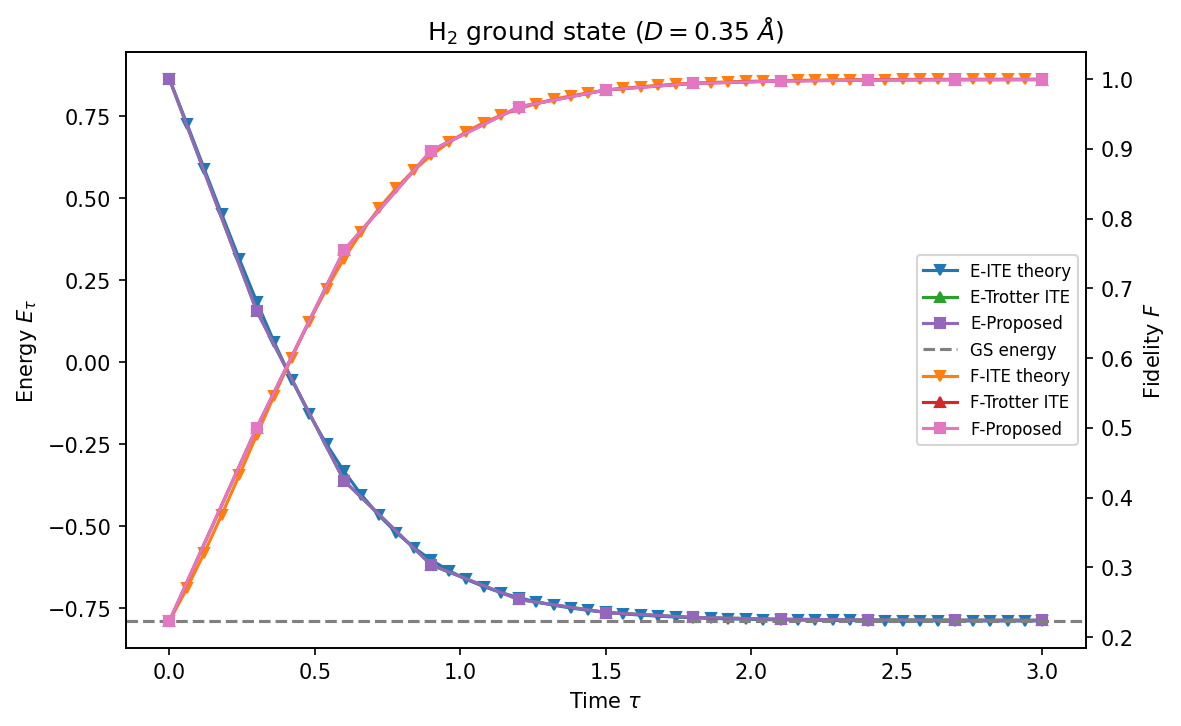
\includegraphics[width=0.85\textwidth]{figure2_h2_convergence.png}
\caption{Energy $E_\tau$ and fidelity $F$ vs.\ imaginary time $\tau$ for H$_2$ at $D = 0.35$~\AA. Three methods are compared: exact ITE (theory), Trotter ITE (no Taylor error), and the proposed TTITE (5th-order Taylor). All converge to the ground state by $\tau \approx 2$.}
\label{fig:h2_convergence}
\end{figure}

\begin{center}
\begin{tabular}{lcc}
\toprule
Quantity & Our code & Paper \\
\midrule
$E_0$ (exact) & $-0.7893$ & $\sim\!-0.85$ \\
$E_\tau$ (TTITE, $\tau=3$) & $-0.7868$ & $\approx E_0$ \\
Fidelity ($\tau=3$) & 0.999 & $\approx 1.0$ \\
\bottomrule
\end{tabular}
\end{center}

\subsection{H$_2$ Molecule: Potential Energy Surface (Figure~3)}

\begin{figure}[h]
\centering
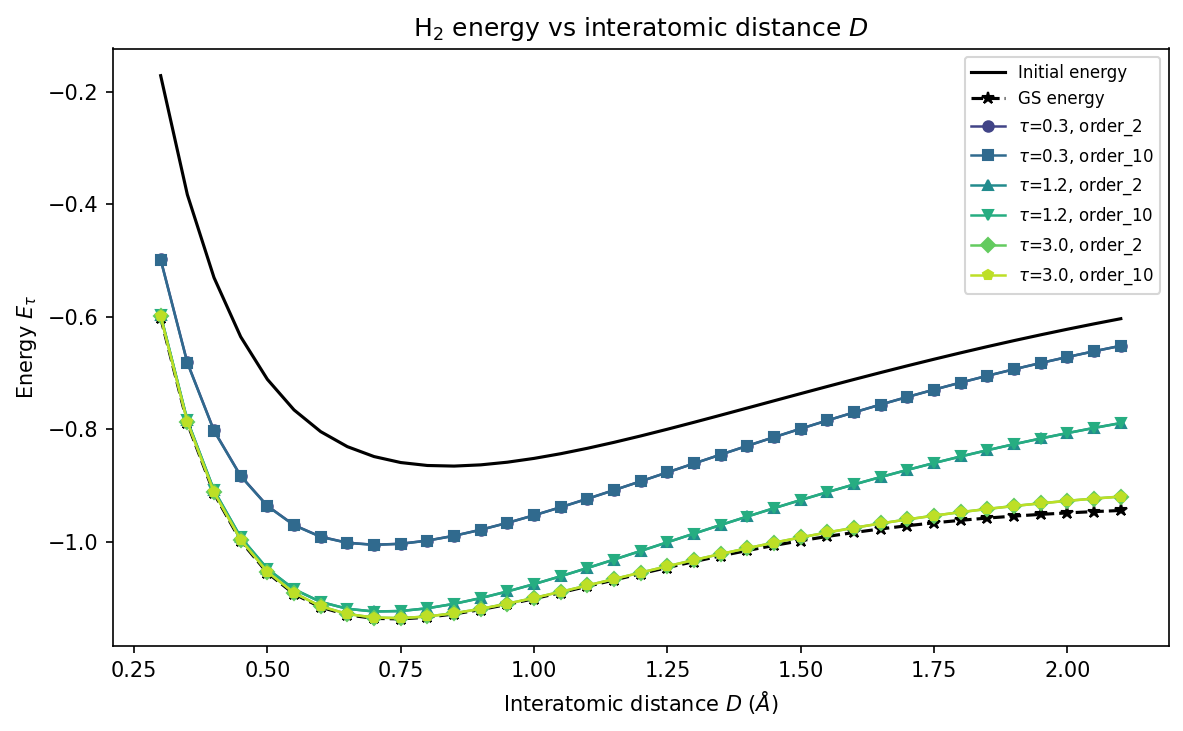
\includegraphics[width=0.85\textwidth]{figure3_h2_pes.png}
\caption{H$_2$ energy after TTITE as a function of interatomic distance $D$, for different $(\tau, R)$ combinations. As $\tau$ increases and/or the Taylor order $R$ increases, the TTITE energy approaches the exact ground state energy (dashed). The PES minimum occurs at $D \approx 0.70$--$0.75$~\AA, consistent with the known equilibrium bond length.}
\label{fig:h2_pes}
\end{figure}

\subsection{Heisenberg Chain: Convergence (Figure~4)}

\begin{figure}[h]
\centering
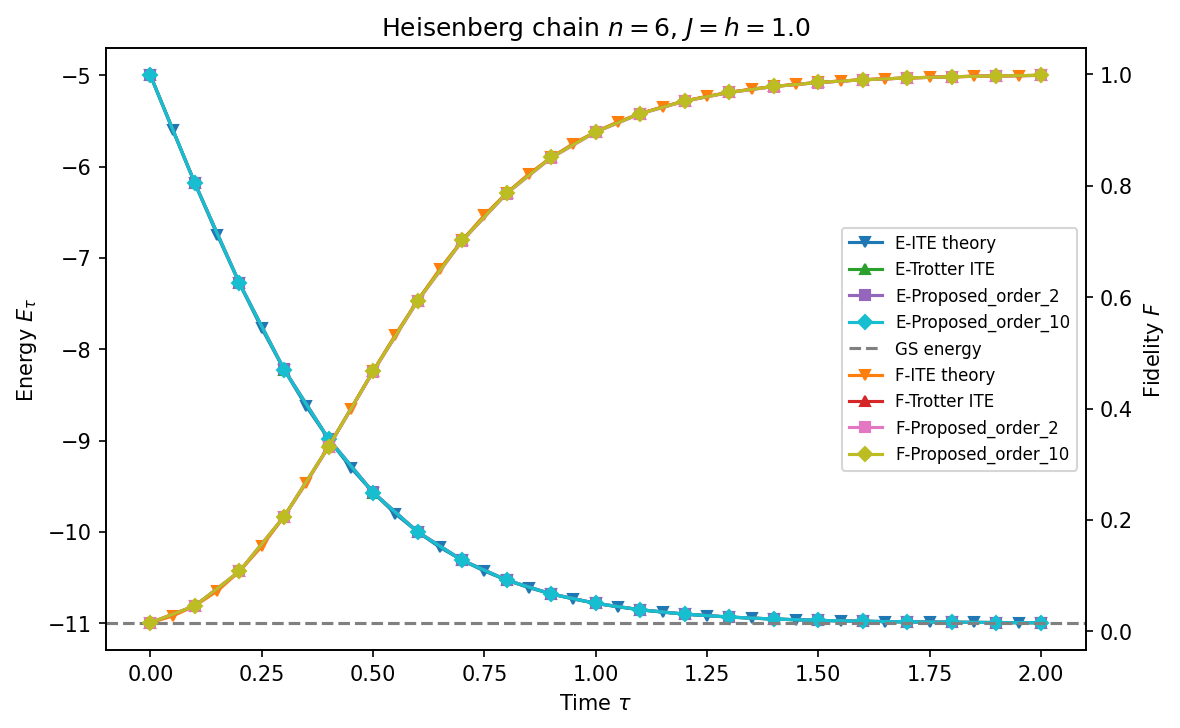
\includegraphics[width=0.85\textwidth]{figure4_heisenberg_convergence.png}
\caption{Heisenberg chain with $n=6$, $J=h=1$. Energy and fidelity converge rapidly. The 2nd and 10th-order Taylor expansions give nearly identical results, confirming that the Taylor error is negligible compared to the Trotter error.}
\label{fig:heisenberg_convergence}
\end{figure}

\subsection{Heisenberg Chain: Scaling (Figure~5)}

\begin{figure}[h]
\centering
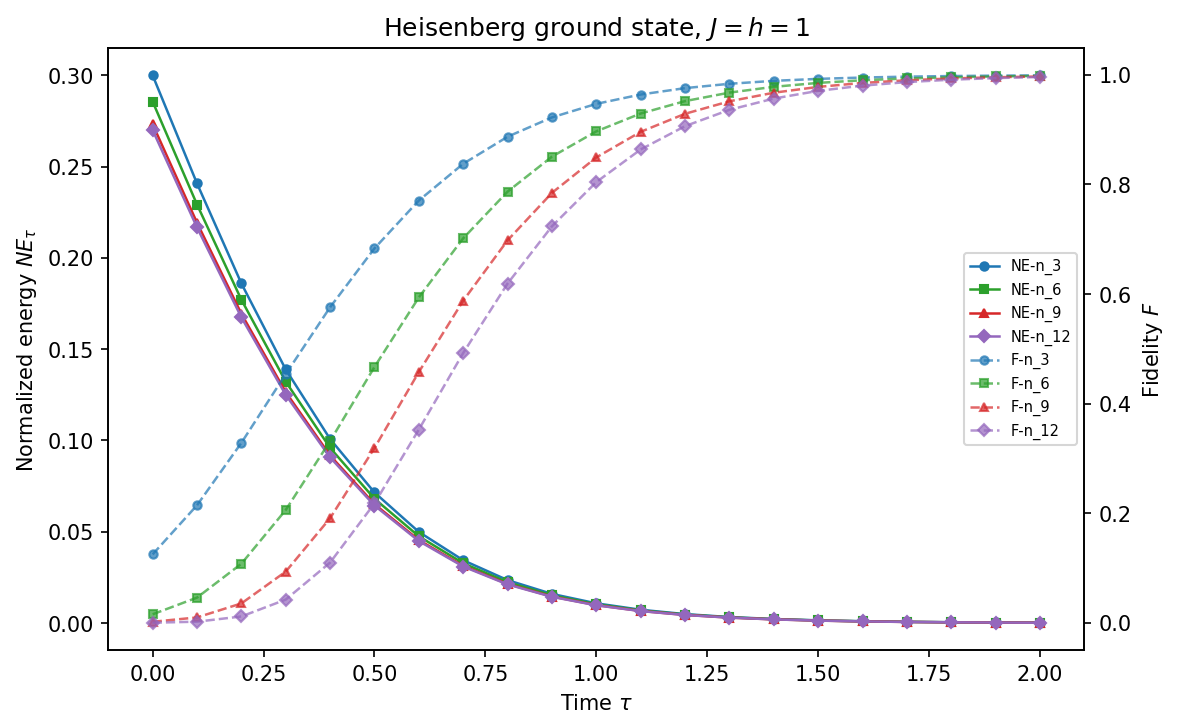
\includegraphics[width=0.85\textwidth]{figure5_heisenberg_scaling.png}
\caption{Normalized energy $NE_\tau = (E_\tau - E_{\min})/(E_{\max} - E_{\min})$ and fidelity $F$ for Heisenberg chains of different sizes ($n = 3, 6, 9, 12$). The algorithm successfully finds the ground state at all sizes, demonstrating scalability.}
\label{fig:heisenberg_scaling}
\end{figure}


%=============================================================================
\section{Code--Equation Mapping}
%=============================================================================

\begin{center}
\begin{tabular}{lll}
\toprule
Paper equation & Code location & Description \\
\midrule
Eq.~(1): $-d\ket{\psi}/d\tau = H\ket{\psi}$ & \texttt{evolution.run\_ite\_exact()} & Exact ITE \\
Eq.~(2): Trotter decomposition & \texttt{evolution.run\_trotter\_ite()} & Trotter ITE \\
Eqs.~(4--5): Taylor expansion & \texttt{circuit.taylor\_coefficients()} & $\alpha, \beta$ coefficients \\
Eq.~(7): Controlled unitary & \texttt{circuit.build\_trotter\_step\_circuit()} & LCU circuit \\
Eq.~(11): Success probability & \texttt{evolution.apply\_trotter\_step\_matrix()} & $P_s$ computation \\
Eq.~(12): H$_2$ Hamiltonian & \texttt{hamiltonian.build\_h2\_hamiltonian()} & 2-qubit H$_2$ \\
Eq.~(13): Heisenberg chain & \texttt{hamiltonian.build\_heisenberg\_hamiltonian()} & $n$-qubit chain \\
Eqs.~(18--20): Improved circuit & \texttt{circuit.build\_improved\_trotter\_step\_circuit()} & Higher $P'_s$ \\
\bottomrule
\end{tabular}
\end{center}


%=============================================================================
\section{Running the Simulation}
%=============================================================================

\begin{lstlisting}[language=bash]
# Install
uv venv && source .venv/bin/activate
uv pip install -e .

# Reproduce all paper figures
python -m quarksim.yihuoliufanzhang.run

# Single figure
python -m quarksim.yihuoliufanzhang.run --figure 2

# Heisenberg chain
python -m quarksim.yihuoliufanzhang.run --system heisenberg --n 6

# Custom parameters
python -m quarksim.yihuoliufanzhang.run --system h2 --D 0.735 --tau 5 --dt 0.1 --order 10
\end{lstlisting}

\textbf{Output files:}
\begin{itemize}[nosep]
  \item \texttt{ttite\_result.json} --- full simulation record
  \item \texttt{figure2\_h2\_convergence.png} --- H$_2$ energy/fidelity convergence
  \item \texttt{figure3\_h2\_pes.png} --- H$_2$ potential energy surface
  \item \texttt{figure4\_heisenberg\_convergence.png} --- Heisenberg convergence
  \item \texttt{figure5\_heisenberg\_scaling.png} --- Heisenberg multi-size scaling
\end{itemize}

\end{document}
